\documentclass[a4paper]{article}
%\usepackage{mathptmx}
\usepackage{amsmath}
\usepackage{amssymb}
\usepackage{amsthm}
%\usepackage[square]{natbib}

\usepackage{tikz}
\usetikzlibrary{positioning}

\newcommand{\arr}{\rightarrow}
\newcommand{\todo}[1]{\bigskip \noindent \emph{todo: #1}}
%\newcommand{\todo}[1]{}

\newtheorem{defNuF}{Definition}[section]
\newtheorem{defNplaceSeparatedSum}[defNuF]{Definition}
\newtheorem{defF}[defNuF]{Definition}
\newtheorem{thmDomNuFisFixedPoint}[defNuF]{Proposition}
\newtheorem{thmDomNuFisFinal}[defNuF]{Proposition}
\newtheorem{defStrictOrderNuF}[defNuF]{Definition}
\newtheorem{defPartialOrderNuF}[defNuF]{Definition}
\newtheorem{thmPONuFisPartial}[defNuF]{Proposition}
\newtheorem{thmPONuFisChainComplete}[defNuF]{Proposition}
\newtheorem{thmPONuFisADomain}[defNuF]{Proposition}
\newtheorem{defIMapsNuFToL}[defNuF]{Definition}
\newtheorem{thmIIsMonotone}[defNuF]{Proposition}
\newtheorem{thmIIsContinuous}[defNuF]{Proposition}

\begin{document}

\title{A domain for the New Naturals}
\author{Markus Klinik}
\maketitle

%\begin{abstract}
%Lorem ipsum.
%\end{abstract}

\section{What are the New Naturals?}


\begin{itemize}
\item Explain inductive data types, F-algebras.
\item Give Examples.
\item Explain coinductive data types, F-coalgebras.
\item Give Examples.
\item The New Naturals are the coinductive data type associated with the
functor $F(X) = 1 + X + X$.
\end{itemize}


Most programming languages offer the possibility to create new data types,
together with functions that operate on them.  In C there are structures, in
Java there are classes, and in contemporary functional programming languages
like Haskell, Clean and OCaml there are algebraic data types.  In this article,
we take a closer look at algebraic data types and their underlying mathematical
ideas.

The definition of an algebraic data type consists of the name of that type,
together with a list of constructors possibly taking parameters.  When supplied
with the correct number and types of arguments, a constructor yields a new
value of that type.

For example, the following piece of Clean code defines a new data type that
could be used to track whether the user of an application has successfully used
the application's authentication functionality before.  The type definition is
to be read as: a user is either a guest or logged in, in which case we know the
username.

\begin{verbatim}
:: User = Guest | LoggedIn String
\end{verbatim}

The first constructor, \verb+Guest+, takes no parameters, and when used as an
expression, it has type \verb+User+.  It can be regarded as a constant value of
type \verb+User+.  The other constructor, \verb+LoggedIn+, takes a
\verb+String+ as its single parameter, so it has type \verb+String -> User+.
In general, each constructor of an algebraic data type $A$ takes some number of
parameters, say n, of type $t_1, t_2, \ldots, t_n$, and the constructor's type
is then the function type that takes all these parameters and yields a value of
the data type: $t_1 \arr t_2 \arr \ldots \arr t_n \arr A$.

\todo{ADTs can be recursive, which means any of the $t_n$ can be A. Trees,
Lists, yadda.}

\todo{Give another example that has the same structure as User, to motivate
different interpretations of inductive types having the same structure.}

When thinking about algebraic data types in general, we're not interested in
names: neither the name of the data type nor the names of the constructors.
What matters is the data type's structure, that is how many different
constructors there are and which type they have.  The idea is similar to lambda
notation, where we denote functions without naming them.

When looking at the above examples of algebraic data types, we can see a
pattern emerge.

The structure of algebraic data types is described with sums of products and
constants.

\section{What is a domain?}

\begin{itemize}
\item A domain is a CPO with a least element.
\item And what is a CPO?  A partial order where every chain has a least upper bound.

\item Finding a domain for the New Naturals means finding a suitable CPO
together with a mapping from the New Naturals to that CPO.

\item We then need to prove that the given construction is indeed a CPO with
least element.

\end{itemize}

\section{Why do we want a domain for the New Naturals?}

\begin{itemize}

\item We want to use the New Naturals in a programming language.

\item We want to be able to reason about this programming language.

\item One way to reason about a programming language is to give it a
denotational semantics and then reason about that.

\item In order to do this, every language construct needs a corresponding
construct in the denotational semantics.

\item Just because we define something, doesn't mean it exists.  Think halting
problem, think Russel's paradox. If we manage to let programs denote domains,
we can apply Tarski's fixed point theorem to be sure that every program has
indeed a valid denotation.

\end{itemize}

\section{A domain for the New Naturals}

\begin{defNplaceSeparatedSum}

The I-place separated sum functor is defined as follows.

\begin{equation}
\sum : \mathbf{Cpo}^I \arr \mathbf{Cpo} \nonumber
\end{equation}

\begin{equation}
\sum_{i \in I}{X_i} =
  \bigcup_{i \in I} \{ \langle i, a \rangle | a \in X_i \}
  \cup \{ \bot \} \nonumber
\end{equation}

\begin{equation}
\sum_{i \in I}{(f_i : X_i \arr Y_i)} :
  \sum_{i \in I}{X_i} \arr \sum_{i \in I}{Y_i}
\end{equation}

\begin{equation*}
(\sum_{i \in I}{f_i)(x)} = \left\{
  \begin{array}{rl}
     \langle i, f(a) \rangle & \text{if } x = \langle i, a \rangle
                               \text{ for some } i \in I \\
    \bot                     & \text{if } x = \bot
  \end{array} \right.
\end{equation*}

\end{defNplaceSeparatedSum}

That is, it takes a family of sets to their disjoint union and adds a bottom
element to the result.  For a family of functions, it applies the corresponding
function to an element of the disjoint union.  We write $\kappa_i(a)$ for
$\langle i, a \rangle$.

Our functor F is then defined as follows.

\begin{defF}
\begin{equation*}
F(X) = \sum{(1, X, X)}
\end{equation*}
\begin{equation*}
F(f : X \arr Y) = \sum{(id_1, f, f)}
\end{equation*}
\end{defF}

\begin{defNuF}

Let $\delta$ be the set of finite and infinite words generated by the following
grammar.

\begin{equation*}
\delta ::= 0 \ |\ \bot \ |\ S \delta \ |\ \_ \delta
\end{equation*}

\end{defNuF}

Among those words are, for example, all peano numbers like $0$, $S0$, $SS0$.
We also have arbitrary underscores mixed in between the successors: $\_0$,
$S\_S\_0$.  Instead of $0$, words can be terminated by $\bot$, e.g.  $S\bot$,
$S\_S\bot$.

Note that all finite words are finite sequences of $S$ and $\_$ which end with
either $0$ or $\bot$. All infinite words are $\omega$-sequences of $S$ and $\_$.
We write $|w|$ to denote the length of a word $w$.

\begin{thmDomNuFisFixedPoint}

The set $\delta$ is a fixed point of the functor $F(X) = 1 + X + X$.

\end{thmDomNuFisFixedPoint}

\begin{proof}

We need to show that $\delta$ is isomorphic to $F(\delta)$, that is, provide two
functions $f : \delta \arr F(\delta)$ and $g : F(\delta) \arr \delta$ such that
their composition is the identity function, i.e. $f \circ g = \text{id}$ and $g
\circ f = \text{id}$.

\end{proof}

\begin{thmDomNuFisFinal}

The set $\delta$ is the largest fixed point for F(X) = 1 + X + X.

\end{thmDomNuFisFinal}

\begin{proof}
What do we need to show?
\end{proof}

\begin{defStrictOrderNuF}

Let the relation $\sqsubset$ on $\delta \times \delta$ be defined as: two
words $s$ and $t$ are in relation $s \sqsubset t$ iff $s$ is finite and $|s|
\leq |t|$ and $s_{|s|-1} = \bot$ and for all $i < |s|-1: s_i = t_i$.

\end{defStrictOrderNuF}


\begin{defPartialOrderNuF}

Let $\sqsubseteq$ be the reflexive closure of $\sqsubset$.

\end{defPartialOrderNuF}


\begin{figure}
\begin{center}
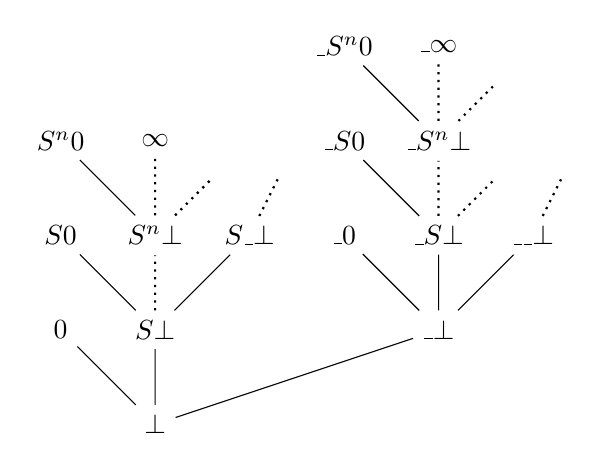
\begin{tikzpicture}
 [ grow'=up
 , scale=1.2
 , level distance=1cm
 , level 1/.style={sibling distance=3cm}
 , level 2/.style={sibling distance=1cm}
 , normal/.style={thin, solid}
 , skipping/.style={thick, dotted}
 , and so on/.style={thick, dotted, sibling distance=0.6cm, level distance=0.6cm}
 ]
  \node {$\bot$}
    child [sibling distance=1cm] { node {$0$} }
    child
    {
      node {$S\bot$}
      child { node {$S0$} }
      child [skipping]
      {
        %node {$SS\bot$}
        %child { node {$SS0$} }
        %child [skipping]
        %{
          node {$S^n\bot$}
          child [normal] { node {$S^n0$} }
          child [skipping] { node {$\infty$} }
          child [and so on] {}
        %}
        %child [and so on] {}
      }
      child
      {
        node {$S\_\bot$}
        child [missing] {}
        child [and so on] {}
      }
    }
    child
    {
      node {$\_ \bot$}
      child { node {$\_0$} }
      child
      {
        node {$\_S\bot$}
        child { node {$\_S0$} }
        child [skipping]
        {
          node {$\_S^n\bot$}
          child [normal] { node {$\_S^n0$} }
          child { node {$\_\infty$} }
          child [and so on] {}
        }
        child [and so on] {}
      }
      child
      {
        node {$\_\_\bot$}
        child [missing] {}
        %child [missing] {}
        child [and so on] {}
      }
    }
  ;
\end{tikzpicture}
\end{center}
\caption{The domain of $\delta$.}
\label{fig:DomainOfNuF}
\end{figure}

The definition of $\sqsubseteq$ is intended to define an information ordering on
$\delta$.  Its relation graph is shown in figure \ref{fig:DomainOfNuF}.
Informally speaking, nodes closer to the root of the tree give less information
than nodes further up the tree.  Consider a process that step-by-step calculates
an element of $\delta$.  We want to interpret the result of the computation
based on the output we have seen so far.  The root node can then be read as ``it
could be any number''.  The value $S\bot$ can be read as ``it is at least one''.
Any value that ends with a $0$ tells us a concrete number, together with the
fact that the process has terminated.  As with flat domains, concrete values are
incomparable, so we don't distinguish between $1$ and $2$ from the viewpoint of
information ordering.

When looking at the subtree of $\_\bot$, we see that its structure is similar
to the whole domain itself, except that every value is prefixed with one additional
underscore.  Nodes in this subtree can be interpreted similarly as described
above, only that it took the process one internal computation step more to
get to this point.

\todo{What's with the sequence of infinite underscores, or a finite number of
sucessors followed by an infinite number of underscores?  Do we regard them as
infinity?}

\todo{Are the two infinities in the picture the same?}

\begin{thmPONuFisPartial}

The relation $\sqsubseteq$ is a partial order.

\end{thmPONuFisPartial}


\begin{proof}

We have to prove the that $\sqsubseteq$ is reflexive, transitive, and
antisymmetric.

Reflexive: by definition.

Transitive: We have to prove that if $s \sqsubseteq t$ and $t \sqsubseteq u$
then $s \sqsubseteq u$ for all words $s$, $t$, $u$. We do so by distinguishing
four cases.

1. If $s = t = u$ then $s \sqsubseteq u$ follows from reflexivity.

2, 3. The cases $s \neq t \wedge t = u \wedge s \sqsubseteq t$ and $s = t
\wedge t \neq u \wedge t \sqsubseteq u$ are trivial.

4. $s \neq t \wedge t \neq u \wedge s \sqsubseteq t \wedge t \sqsubseteq u$ We
have: $|s| \leq |t| \leq |u|$ and $s_{|s|-1} = \bot$ and $t_{|t|-1} = \bot$ and
for all $i < |s|-1: s_i = t_i$ and for all $j < |t|-1: t_j = u_j$.  But this
means, because of $|s| \leq |t|$: for all $i < |s|-1: s_i = u_i$, hence $s
\sqsubseteq u$.

Antisymmetric: We have to prove that if $s \sqsubseteq t \wedge t \sqsubseteq
s$ then $s = t$.  The premise is either the case because $s = t$ to begin with,
or we have: $s$ is finite and $|s| \leq |t|$ and $s_{|s|-1} = \bot$ and for all $j <
i: s_j = t_j$ and $t$ is finite and $|t| \leq |s|$ and $t_{|t|-1} = \bot$ and for all
$j < i: t_j = s_j$.  But then $s$ and $t$ are both finite, of the same length,
and agree in all elements, hence $s = t$.

\end{proof}

\begin{thmPONuFisChainComplete}

The relation $\sqsubseteq$ is chain complete.

\end{thmPONuFisChainComplete}

We need to show that every $\omega$-chain in $\delta$ has a least upper bound.
An $\omega$-chain in $\delta$ is a sequence $f : \mathbb{N} \arr \delta$ such
that for all $i \in \mathbb{N}: f(i) \sqsubseteq f(i + 1)$.


\begin{thmPONuFisADomain}

The structure $(\delta, \sqsubseteq)$ is a domain.

\end{thmPONuFisADomain}

We need to show that $(\delta, \sqsubseteq)$ has a least element, i.e. there is
an element $s \in \delta$ such that for any other element $t \in \delta: s
\sqsubseteq t$.

Next, we want to check if we can recover the lazy natural numbers, denoted by
$L$, from the New Naturals by giving a continuous map between $\delta$ and $L$.
The domain $(L, \sqsubseteq)$ is given informally in figure
\ref{fig:DomainOfLazyNaturals}.

%\begin{figure}
%\begin{center}
%\begin{tikzpicture}
  %\node {$\underline 0$} [grow'=up, sibling distance=4.0em, level distance=1.8em]
    %child { node {$0$} }
    %child
    %{
      %node {$\underline 1$}
      %child { node {$1$} }
      %child
      %{
        %node {$\underline 2$}
        %child { node {$2$} }
        %child [thick, dotted]
        %{
          %node {$\underline n$}
          %child [thin, solid] { node {$n$} }
          %child { node {$\infty$} }
        %}
      %}
    %}
  %;
%\end{tikzpicture}
%\end{center}
%\caption{The domain of the lazy natural numbers.}
%\label{fig:DomainOfLazyNaturals}
%\end{figure}

\begin{figure}
\begin{center}
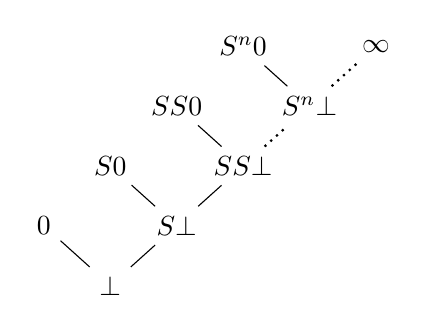
\begin{tikzpicture}[scale=1.2]
  \node {$\bot$} [grow'=up, sibling distance=4.0em, level distance=1.8em]
    child { node {$0$} }
    child
    {
      node {$S\bot$}
      child { node {$S0$} }
      child
      {
        node {$SS\bot$}
        child { node {$SS0$} }
        child [thick, dotted]
        {
          node {$S^n\bot$}
          child [thin, solid] { node {$S^n0$} }
          child { node {$\infty$} }
        }
      }
    }
  ;
\end{tikzpicture}
\end{center}
\caption{The domain of the lazy natural numbers.}
\label{fig:DomainOfLazyNaturals}
\end{figure}

\begin{defIMapsNuFToL}

Define the function $I : \delta \arr L$ as follows: \ldots

\end{defIMapsNuFToL}


\begin{thmIIsMonotone}

The function $I$ is monotone.

\end{thmIIsMonotone}


\begin{thmIIsContinuous}

The function $I$ is continuous.

\end{thmIIsContinuous}

\section{Further directions}

\begin{itemize}
\item Embed the New Naturals into some coinductive PCF.
\item Analyze if the domain composes nicely (or at all) with the other
denotations.
\item Can we generalize the construction of the domain to arbitrary
F-coalgebras?
\end{itemize}

\section{Bibliographic notes}

Lorem ipsum \cite{Pierce1991} \cite{Gunter1992} \cite{Bird1997}
\cite{Mitchell1996} \cite{Allison1986} \cite{Capretta2002}

\bibliographystyle{plain}
\bibliography{computer_science}
\end{document}

% vim: textwidth=80
